\chapter{Data Acquisition System for the Focal-Plane Detector Package}
\label{ch:DAQ}

%%%%%%%%%%%%%%%%%%%%%%%%%%%%%%%%%%%%%%%%%%%%%%%%%%%%%%%%%%%%%%%%%%%%%%%%%%%%%%%

\section{Introduction}

A new digital data acquisition system (DAQ) and graphical user interface (GUI) have been developed for use with the focal-plane detector package \cite{Marshall2019} of the Enge Split-Pole Spectrograph at the Triangle Universities Nuclear Laboratory (TUNL). The CAEN V1730 digitizer is meant to replace the traditional analog modules and analog-to-digital converter (ADC) that have previously been used for the focal-plane detector.

The purpose of this document is twofold. Firstly, it serves as an operation manual on the components of our upgraded system - the CAEN V1730 digitizer (Section 3), our custom frontend DAQ software (Section 4), and our custom GUI: EngeSpec (Section 5). Secondly, it provides a record of the author's contributions to the development of the DAQ (Section 4) and the GUI (Section 5) and to testing the new system with live data (Section 6). Section 2 provides a brief background and motivates the need for the upgrades.

%system (DAQ) and graphical user interface (GUI)

%%%%%%%%%%%%%%%%%%%%%%%%%%%%%%%%%%%%%%%%%%%%%%%%%%%%%%%%%%%%%%%%%%%%%%%%%%%%%%%

\pagebreak
\section{Background and Motivation} \label{motivation}

% Note: "Analog DAQ" is probably not a thing. Instead, have this part be about Analog Modules vs. Digitizers. The "DAQ" should only refer to the custom DAQ software, i.e. the digitizer and its firmware are not part of the DAQ, nor is the EngeSpec GUI.

Nuclear physics experiments involving the detection of radiation ($\gamma$-rays, neutrons, protons, $\alpha$-particles, etc.) require a method of converting detected radiation into numerical data. 
%The DAQ is responsible for collecting, processing, sorting, storing, and visualizing events from radiation detectors.
%\footnote{Some define the term DAQ as being associated with only the collection, sorting, and storing of data, while processing and visualizing are separate functions reserved for signal-processing modules and GUIs, respectively. Here, we define a DAQ system as the entire process of acquiring data.}. 
Figure \ref{traditional_electronics} illustrates the components of the traditional data acquistion method. Detectors first convert each radiation event into an analog electrical signal, or pulse. Pulse processing then alters the detector signal so as to reduce noise and amplify the pulse to sufficiently measurable levels. At this point, the energy and timing of the event can be determined by further processing. This processing is traditionally performed by a network of analog modules, where the processed pulse is then converted to a digital pulse via an analog-to-digital converter (ADC). The digital pulse can finally be read by a computer and collected by a data acquisition (DAQ) software. The stored data can be visualized by a graphical user interface (GUI), which sorts all of the data based on the corresponding detectors and observables, displays histograms, and can perform a number of functions, such as curve fitting and gating.

\begin{figure}[b!]
\centering
\begin{tikzpicture}[scale=0.96, every node/.style={transform shape}]

\node at (-2.5,0) {
\includegraphics[scale=0.03]{Chapter-5/figs/radiation.png}};
\node at (-2.5,-0.75) {\footnotesize{Radiation}};
\draw[->] (-1.8,0) -- (-1.3,0);
\node[cylinder, draw, shape aspect=0.5, minimum height=0.5cm, scale=2,cylinder uses custom fill,cylinder body fill=gray!50,cylinder end fill=gray!25,rotate=180]{};
\begin{scope}[shift={(-0.6,0)}]
\node[cylinder, draw, shape aspect=0.5, minimum height=0.001cm, scale=1,cylinder uses custom fill,cylinder body fill=gray!50,cylinder end fill=gray!25,rotate=180]{};
\end{scope}
\node at (-0.2, -0.75) {\footnotesize{Detector(s)}};

%\node at (-0.25,-2.5) {\includegraphics[scale=0.08]{detector_signal}};
%\draw[->] (-0.2, -1.1) -- (-0.2, -1.6);
%\node at (-0.2, -3.5) {\footnotesize{Signal}};

\node at (1.05,-2.5) {\includegraphics[scale=0.08]{Chapter-5/figs/detector_signal.png}};
\draw[->] (1.05, -0.5) -- (1.05, -1.6);
\node at (1.05, -3.5) {\footnotesize{Signal}};

\draw[->] (0.8,0) -- (1.3,0);
\node at (2.7, -1.4) {\footnotesize{Analog Modules}};

\filldraw[fill=brown!70] (1.8,-1) rectangle (2.1,1);
\filldraw[fill=brown!70] (2.3,-1) rectangle (2.6,1);
\filldraw[fill=brown!70] (2.8,-1) rectangle (3.1,1);
\filldraw[fill=brown!70] (3.3,-1) rectangle (3.6,1);

\coordinate (A) at (1.45,-0.8,0);
\coordinate (B) at (1.95,0.8);
\coordinate (C) at (1.95,-0.8);
\coordinate (D) at (2.45,0.8);
\coordinate (E) at (2.45,-0.8);
\coordinate (F) at (2.95,0.8);
\coordinate (G) at (2.95,-0.8);
\coordinate (H) at (3.45,0.8);
\coordinate (I) at (3.45,-0.8);
\coordinate (J) at (3.95,0.8);

\filldraw[fill = white] (B) circle (0.5mm);
\filldraw[fill = white] (C) circle (0.5mm);
\filldraw[fill = white] (D) circle (0.5mm);
\filldraw[fill = white] (E) circle (0.5mm);
\filldraw[fill = white] (F) circle (0.5mm);
\filldraw[fill = white] (G) circle (0.5mm);
\filldraw[fill = white] (H) circle (0.5mm);
\filldraw[fill = white] (I) circle (0.5mm);

\draw (A) to [bend right = 10] (B);
\draw (C) to [bend right = 10] (D);
\draw (E) to [bend right = 10] (F);
\draw (G) to [bend right = 10] (H);
\draw (I) to [bend right = 10] (J);

\draw[->] (4.1,0) -- (4.6,0);
\filldraw[fill=black!50] (5,-1) rectangle (5.3,1);
\filldraw[fill = white] (5.15, 0.8) circle (0.5mm);
\filldraw[fill = white] (5.15, -0.8) circle (0.5mm);
\draw (4.65, -0.8) to [bend right = 10] (5.15, 0.8);
\draw (5.15, -0.8) to [bend right = 10] (5.65, 0.8);
\node at (5.15,-1.4) {\footnotesize{Analog}};
\node at (5.15,-1.75) {\footnotesize{to Digital}};
\node at (5.15,-2.05) {\footnotesize{Converter}};

\draw[->] (5.8,0) -- (6.3,0);
\node at (7.8,0) {
\includegraphics[scale=0.1]{Chapter-5/figs/computer_screen.png}};
\node at (7.8,-1.35) {\footnotesize{Computer / GUI /}};
\node at (7.8,-1.7) {\footnotesize{DAQ Software}};

\draw[->] (7.8, -1.9) -- (7.8, -2.4);
\node at (7.8,-3.4) {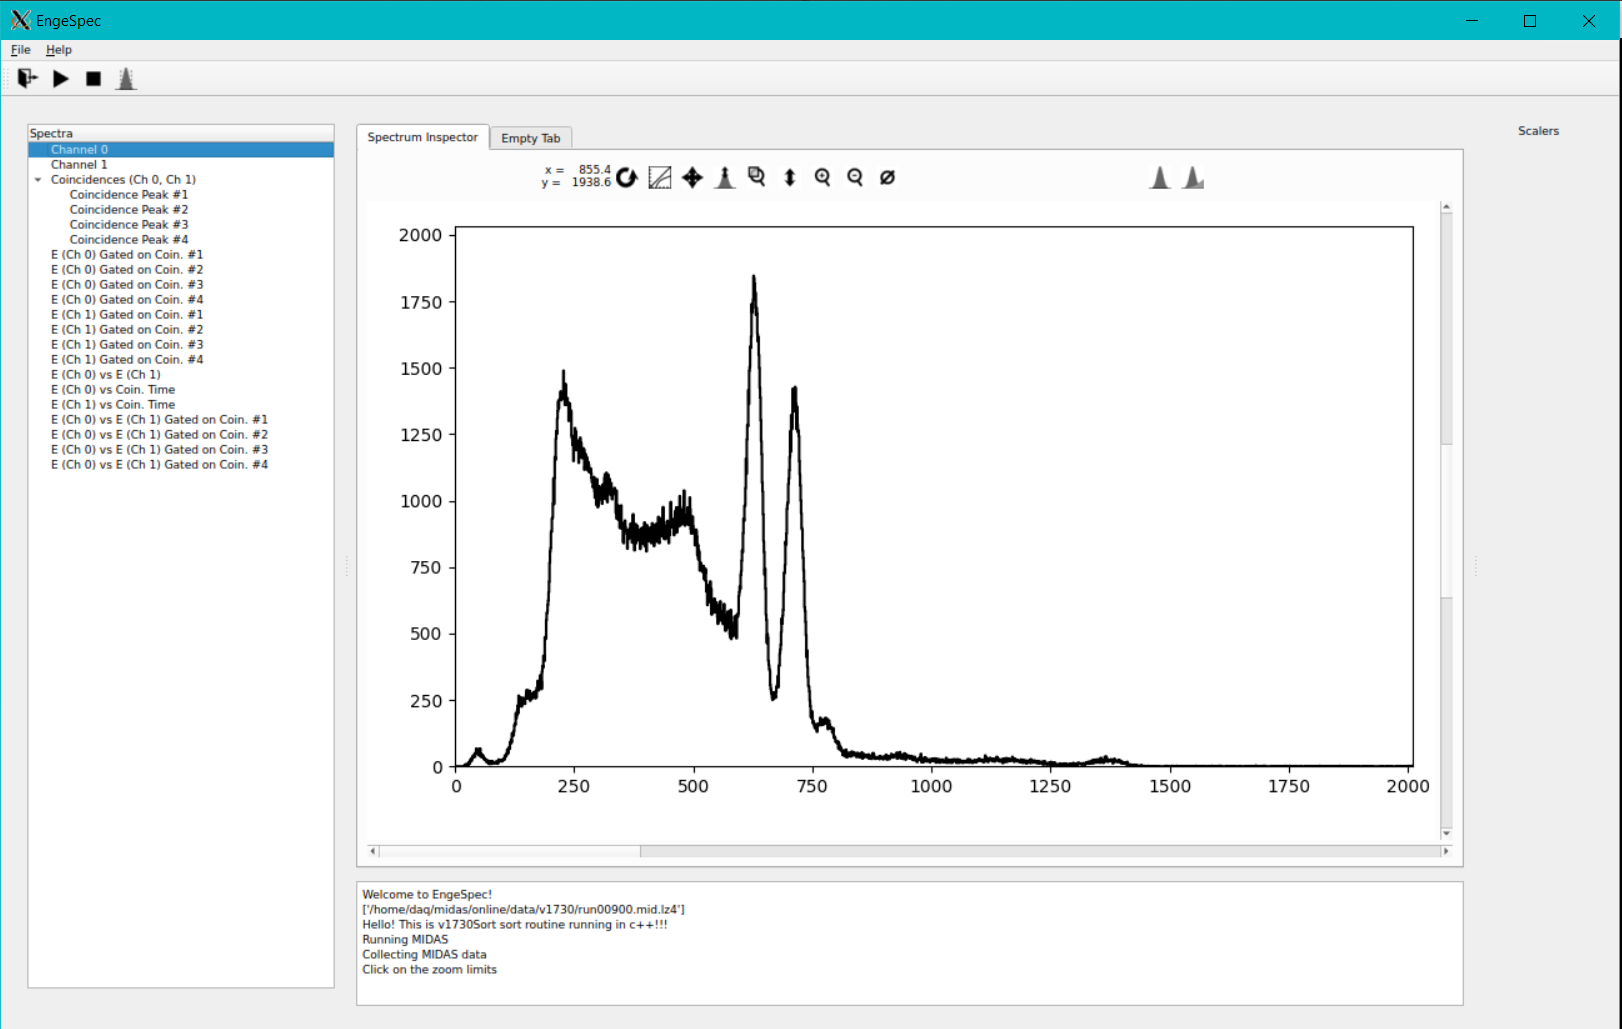
\includegraphics[scale=0.08]{Chapter-5/figs/Histogram_Co60.png}};
\node at (7.8,-4.5) {\footnotesize{Numerical Data}};

%\draw[decorate,decoration={brace,amplitude=5pt},rotate=270] (2.55,4.75) -- (2.55,3.25);
%\draw[decorate,decoration={brace,amplitude=5pt},rotate=270] (2.35,7.5) -- (2.35,3.25);
%\node at (4.3,-2.95) {Upgrading for};
%\node at (4.3,-3.25) {$^{87}\textnormal{Rb} + \gamma$ experiments};
%\draw[red] (2.5, -3.5) rectangle (6.1,-2.7);

\end{tikzpicture}
\caption{The traditional method of converting detected radiation into numerical data using analog pulse-processing modules and an analog-to-digital converter (ADC).}
\label{traditional_electronics}
\end{figure}

The network of analog pulse-processing modules needed for nuclear physics experiments can be incredibly complex. Input and output cables connect modules together, and the vast number of cables can be cumbersome. Rearranging the network of modules between experiments amounts to physically altering the cable setup, which can lead to cable-mapping issues. The modules themselves also take up a significant amount of space. Hence, analog modules have an inherent portability problem.

A network of traditional analog modules can be replaced by a single digitizer, a module that performs the same pulse processing digitally after it samples the detector signals itself. Figure \ref{new_electronics} illustrates the new data acquisition method using a digitizer instead of analog modules and an ADC. Digitizers use firmware algorithms to emulate the functions of analog modules. Custom software is written by the user to perform specific functions that are needed for a given experiment. Changing the setup between experiments now amounts to altering existing code, rather than moving physical equipment. 

At TUNL, the Longland group is replacing the focal-plane detector's analog modules with the CAEN V1730 digitizer and its associated Digital Pulse Processing (DPP) firmware algorithms. Figure \ref{upgrade} shows the difference between the old analog module setup versus the digitizer. Portability will now be significantly improved, and a large amount of physical space will be freed up for other purposes. The 14-bit digitizer will also provide enhanced energy and timing resolutions compared to the previous 12-bit ADC.

We have written a custom frontend DAQ software to accompany the digitizer, which uses MIDAS (Maximum Integrated Data Acquistion System) as our event-based DAQ. The DAQ software we used for our old system, NSCLDAQ, will no longer be supported soon, which is another incentive for the upgrades. In order to visualize the data from our new digitizer and DAQ, we have developed a GUI, called EngeSpec, that is connected with MIDAS to provide live data visualization during experiments. It also has an offline mode for analysis with previously stored data. EngeSpec has several data analysis tools like curve fitting for Gaussian and double-Gaussian peaks, peak area calculation, and gating functionality. A sort routine, called EngeSort, that was used with the old GUI has been revamped for use with EngeSpec. As before, it sorts the data by detector channel and by observable into each given histogram. However, the new EngeSort includes trigger and coincidence logic for the Enge focal-plane detector package, something that was previously performed by analog modules.

\begin{figure}[t!]
\centering
\begin{tikzpicture}[scale=0.96, every node/.style={transform shape}]
\hspace{-0.6cm}

\hspace{1.6cm}
\node at (-2.5,0) {
\includegraphics[scale=0.03]{Chapter-5/figs/radiation.png}};
\node at (-2.5,-0.75) {\footnotesize{Radiation}};
\draw[->] (-1.8,0) -- (-1.3,0);
\node[cylinder, draw, shape aspect=0.5, minimum height=0.5cm, scale=2,cylinder uses custom fill,cylinder body fill=gray!50,cylinder end fill=gray!25,rotate=180]{};
\begin{scope}[shift={(-0.6,0)}]
\node[cylinder, draw, shape aspect=0.5, minimum height=0.001cm, scale=1,cylinder uses custom fill,cylinder body fill=gray!50,cylinder end fill=gray!25,rotate=180]{};
\end{scope}
\node at (-0.2, -0.75) {\footnotesize{Detector(s)}};

\node at (1.05,-2.5) {\includegraphics[scale=0.08]{Chapter-5/figs/detector_signal.png}};
\draw[->] (1.05, -0.5) -- (1.05, -1.6);
\node at (1.05, -3.5) {\footnotesize{Signal}};

\draw[->] (0.8,0) -- (1.3,0);
%\node at (2.7, -1.4) {\footnotesize{Analog Modules}};
%\draw[->] (4.1,0) -- (4.6,0);

\hspace{-1.6cm}

\hspace{-1.6cm}
\filldraw[fill=red!50] (5,-1) rectangle (5.3,1);
\filldraw[fill = white] (5.15, 0.8) circle (0.5mm);
\filldraw[fill = white] (5.15, -0.8) circle (0.5mm);
\draw (4.65, -0.8) to [bend right = 10] (5.15, 0.8);
\draw (5.15, -0.8) to [bend right = 10] (5.65, 0.8);
\node at (5.15,-1.4) {\footnotesize{Digitizer}};
\hspace{1.6cm}

\hspace{-1.6cm}
\draw[->] (5.8,0) -- (6.3,0);
\node at (7.8,0) {
\includegraphics[scale=0.1]{Chapter-5/figs/computer_screen.png}};
\node at (7.8,-1.35) {\footnotesize{Computer / GUI /}};
\node at (7.8,-1.7) {\footnotesize{Custom DAQ Software}};

\draw[->] (7.8, -1.9) -- (7.8, -2.4);
\node at (7.8,-3.4) {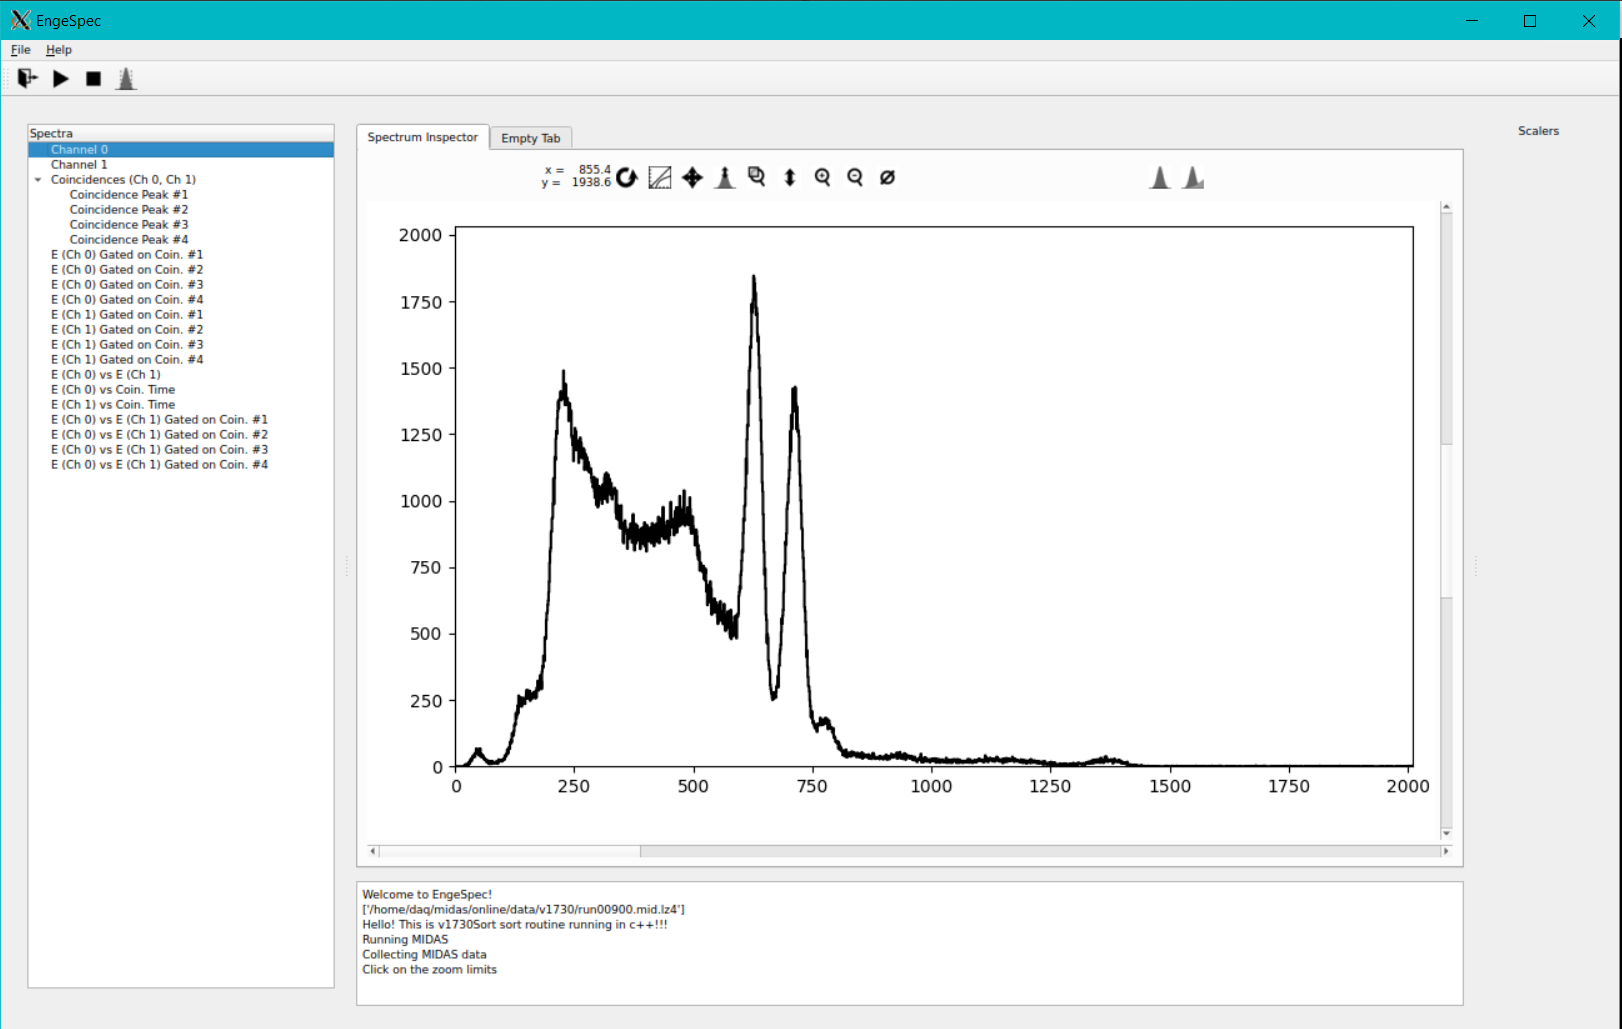
\includegraphics[scale=0.08]{Chapter-5/figs/Histogram_Co60.png}};
\node at (7.8,-4.5) {\footnotesize{Numerical Data}};
\hspace{1.6cm}

\end{tikzpicture}
\caption{The new method of converting detected radiation into numerical data with a digitizer, which replaces analog modules.}
\label{new_electronics}
\end{figure}

\pagebreak

\textcolor{white}{Empty space to force figure to top...}

\begin{figure}[t]
\centering
\begin{tikzpicture}
\hspace{0.3cm}
\node at (-3,0) {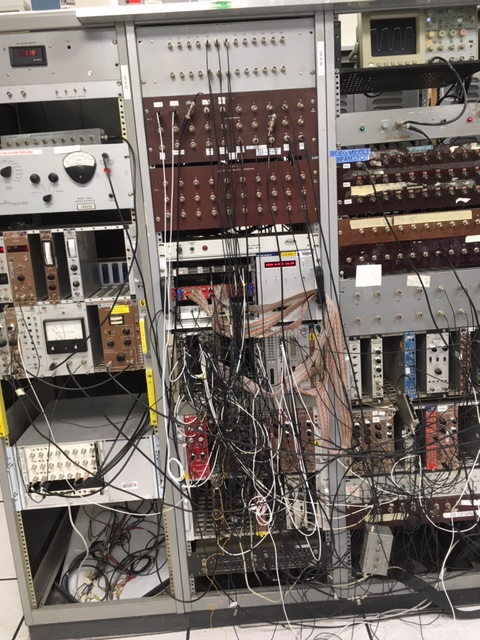
\includegraphics[scale=0.3]{Chapter-5/figs/Analog_Electronics.png}};
\node at (-3,-2.9) {\small{Analog Modules}};
\draw[->] (-0.5,0) -- (0.5,0);
\node at (0, 0.4) {\footnotesize{Upgrading}};
\node at (3,0) {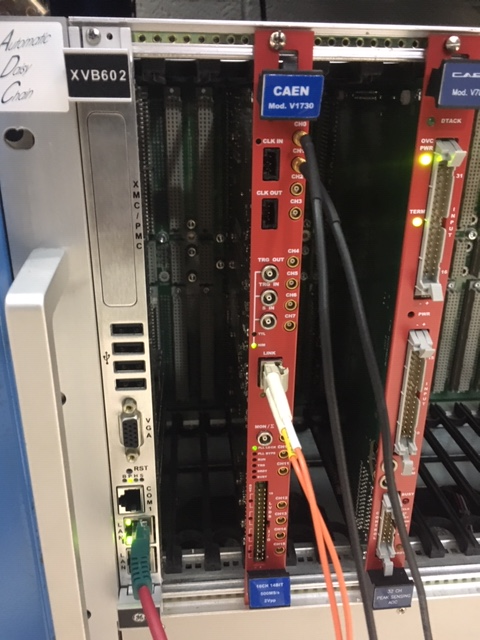
\includegraphics[scale=0.3]{Chapter-5/figs/Digitizer.png}};
\filldraw[fill = white] (4.1,-2.4) rectangle (5.9,-1.9);
\node at (5, -2.15) {\small{+ Software}};
\node at (3, -2.9) {\small{Digitizer}};
\end{tikzpicture}
\caption{The CAEN V1730 Digitizer (pictured on the right), along with its associated DPP firmware and custom frontend DAQ software, is replacing the need for the unportable analog pulse-processing modules (pictured on the left) associated with the Enge focal-plane detector package at TUNL.}
\label{upgrade}
\end{figure}

%%%%%%%%%%%%%%%%%%%%%%%%%%%%%%%%%%%%%%%%%%%%%%%%%%%%%%%%%%%%%%%%%%%%%%%%%%%%%%%

\clearpage % This doesn't seem to separate the section because of the last figure
\section{Overview of the CAEN V1730 Digitizer} \label{digitizer} 

This section provides a brief overview of how the CAEN V1730 digitizer functions, where the most important aspects of its Digital Pulse Processing (DPP) algorithms are discussed. Section \ref{frontend} covers how to implement the algorithms via our frontend DAQ software. Our version of the digitizer firmware is known as DPP-PSD, or Digital Pulse Processing for Pulse Shape Discrimination. The official CAEN DPP-PSD user manual \textcolor{blue}{[Ref]} %\ref{CAEN DPP-PSD user manual} 
is a comprehensive reference for details not covered in this document. 

%One of the main features of our version of the firmware is Pulse Shape Discrimination (PSD), which allows the user to distinguish between, for example, $\gamma$-ray and neutron events. Hence, it is known as the DPP-PSD firmware. The official CAEN DPP-PSD user manual is a useful reference for details not covered in this document.

\subsection{Digital Pulse-Processing Parameters} \label{DPP}

\begin{figure}[b!]
\centering
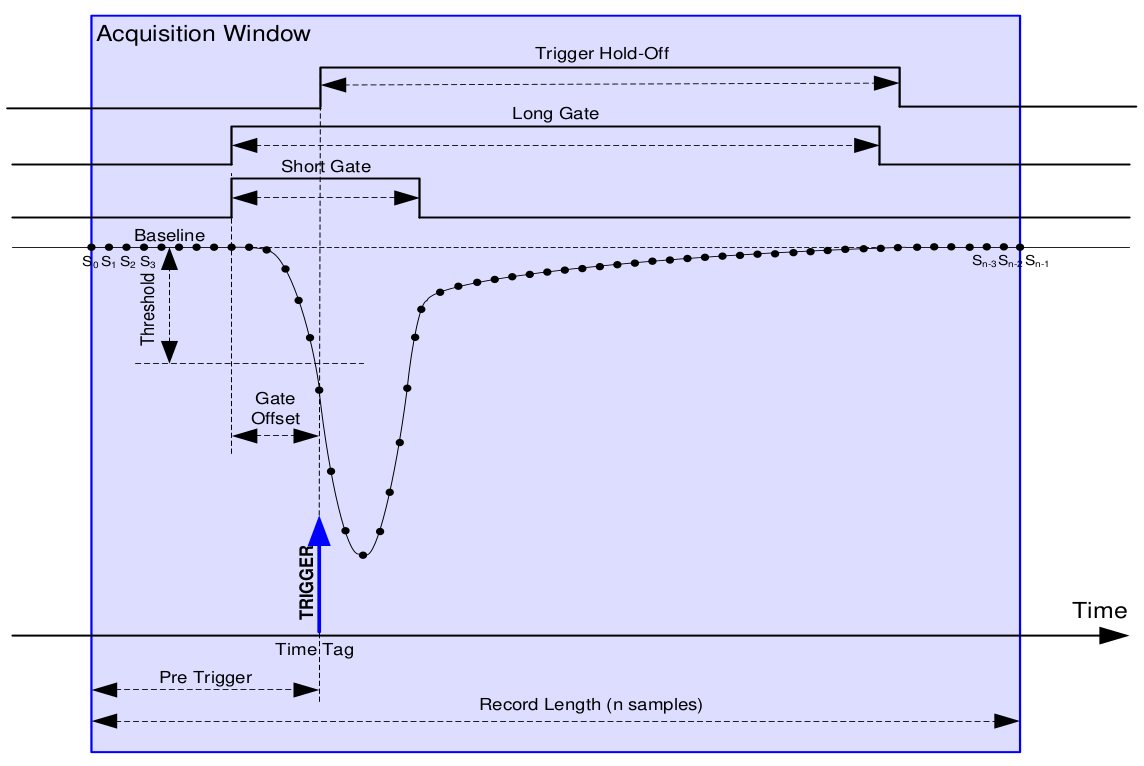
\includegraphics[scale=0.3]{Chapter-5/figs/trigger.png}
\caption{A signal sampled by the V1730 digitizer, summarizing the parameters used by the DPP algorithms. When the signal crosses the threshold value, the trigger fires, which primes the system for data acquisition.}
\label{trigger}
\end{figure}

The V1730 digitizer is capable of sampling signals directly from detectors at a rate of 500 MS/s for each of its 16 input channels, corresponding to a time resolution of 2 ns per sample. Those samples are used by the DPP firmware in calculations of important quantities associated with a given signal, such as its baseline, energy, and time stamp. A typical sampled signal is shown in Figure \ref{trigger}, where parameters used by the DPP algorithms are summarized. These parameters are all user-defined and depend on the shape of the detector signals. One can use an oscilloscope or any waveform display software, such as CoMPASS, to approximate the parameters. For optimal resolution, it may be necessary to perform resolution tests for certain parameters over a range of values (see Section \ref{resolution} for an example).

%\subsubsection{Energy Calculation} \label{energy_calc}

A signal is triggered for data acquisition when it crosses the \textit{threshold} voltage, which should be set high enough to filter out low-energy noise. When the trigger fires, the signal is delayed by the \textit{pre-trigger} width to prime for the energy calculation. Since the energy of a radiation event is proportional to the charge that it deposits, the digitizer calculates this charge, and therefore determines the (uncalibrated) energy, by integrating the signal voltage over time. The length of time used in the integration is a user-defined parameter known as the \textit{long gate}, and the integrated charge (i.e. uncalibrated energy) is denoted by $Q_{\textnormal{Long}}$. The energy integration begins a length of time before the trigger fires, known as the \textit{gate offset}, which must be less than the pre-trigger width. The purpose of the gate offset is to include the portion of the signal before the trigger in the energy integration. After the trigger fires, all other triggers from the same channel are inhibited during the \textit{trigger hold-off} width, which must last at least until the end of the long gate. After this width, the channel can accept new triggers. 

%Q: HOW DO EVENTS THAT ARE COINCIDENT EVEN GET TRIGGERED WHEN THEY SHOULD BE INHIBITED DURING THE TRIGGER HOLD-OFF WIDTH? 
%A: BECAUSE THE EVENTS THAT ARE COINCIDENT COME FROM DIFFERENT CHANNELS WITH THEIR OWN TRIGGER HOLD-OFF.

\begin{figure}[b!]
\centering
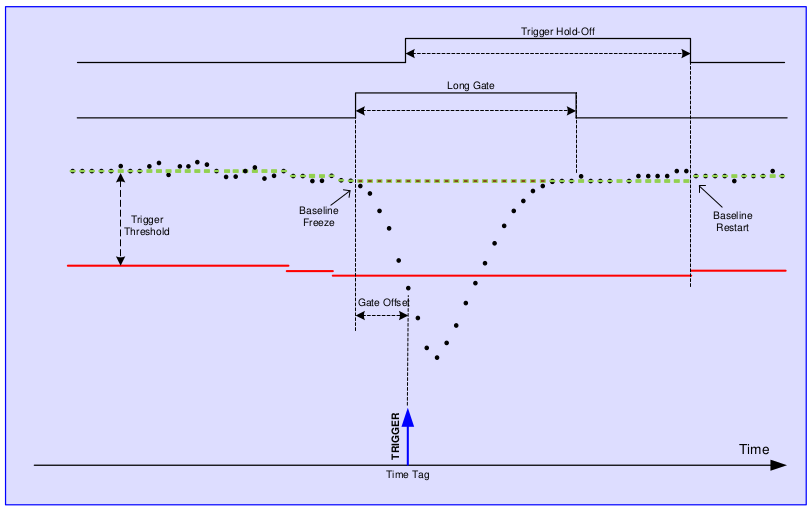
\includegraphics[scale=0.38]{Chapter-5/figs/baseline.png}
\caption{The dynamic baseline calculation using the mean value of a user-defined number of samples in a moving time window. The baseline freezes during the energy integration of a signal that has been triggered.}
\label{baseline_calc}
\end{figure}

One of the most important quantities associated with the DPP algorithms is the baseline of the signal. The baseline is the reference value used for the energy calculation and to determine the threshold. This can either be a user-defined quantity, in which case it retains a fixed value, or the baseline can be dynamically calculated based on the average value of a user-defined number of samples during a moving time window (see Section \ref{mean_baseline_calc} for the specific options). In the latter case, as shown in Figure \ref{baseline_calc}, the baseline freezes during energy integration, and the baseline calculation restarts after the trigger hold-off width, using the samples both before and after the freeze. This means the baseline calculation contributes almost no dead-time. Note that the threshold follows the baseline variations.

The \textit{short gate} is a measure of the fast portion of the signal. This is used, in conjunction with the long gate, to discern between different types of particles, e.g. between gamma-rays and neutrons. The pulse shape discrimination (PSD) is a quantity that measures the ratio between the area of the tail of the signal and the area of the total signal, i.e.
\begin{equation*}
\textnormal{PSD} = \frac{Q_{\textnormal{Long}} - Q_{\textnormal{Short}}}{Q_{\textnormal{Long}}},
\end{equation*}
where $Q_{\textnormal{Long}}$ and $Q_{\textnormal{Short}}$ are the charge collected in the long gate and short gate during charge integration, respectively. Neutron events tend to have a distinctly higher PSD than gamma-ray events because they have larger tails. The option to collect the PSD for each event is not yet available in our frontend software, but it will be added soon.

The only parameter yet to be discussed in Figure \ref{trigger}, the \textit{record length}, is not used by our digitizer. The V1730 only operates in List mode, where the event data is stored, but the samples themselves are not. Some other CAEN digitizers can operate in Waveform mode, where the samples in the record length that make up the \textit{acquisition window} are stored to visualize the signals and the baseline with the appropriate CAEN software. However, the reduced amount of data transferred in List mode compared to Waveform mode keeps the dead-time of the system very low during runs.

\subsection{Time Stamp Determination} \label{time_stamp}

%\subsubsection{Leading Edge Discrimination} \label{LED}

By default, the timing of events in the DPP firmware is performed by \textit{leading edge discrimination} (LED), where a time stamp is given to each event the moment it crosses the trigger threshold. However, threshold triggering on the leading edge of signals causes well-known issues with timing, known as \textit{time walk}. Two signals exactly coincident, but with different amplitudes, will register different time tags using LED mode because the leading edge of the larger signal rises sooner. 

%\subsubsection{Constant Fraction Discrimination} \label{CFD}

A more precise way of determining signal time is by using \textit{constant fraction discrimination} (CFD), which can be enabled by the DAQ user instead of LED mode (see Section \ref{LED_CFD}). This method assigns the time stamp to the moment the signal amplitude reaches a constant fraction of its total amplitude, allowing for timing to be independent of signal amplitude. As in traditional analog CFD modules, the digitizer takes the input signal and produces two new signals, one attenuated by a factor $f$ of the total amplitude and the other inverted and delayed by a time $d$. The two signals are summed together to form a bipolar pulse with a single \textit{zero-crossing}, which is taken as the time stamp of the event. Because of the finite sampling resolution of the digitizer, the exact zero-crossing location will always be located somewhere between two samples of the signal. The DPP firmware, by default, assigns the sample before the zero-crossing as the time stamp of the event, called the \textit{coarse time stamp}. This is usually sufficient, but for more precise timing it is also possible to assign the time stamp as the interpolated zero-crossing. The width between the coarse time stamp and the interpolated zero-crossing is called the \textit{fine time stamp}. If the user enables zero-crossing interpolation, the data for each event will take up more memory. Note that in the case of CFD mode, the threshold trigger serves the purpose of priming the system for CFD implementation rather than assigning a time stamp.

The time stamp for LED mode and the coarse time stamp for CFD mode are both referred to as the \textit{trigger time tag} in the DPP firmware, a 31-bit unsigned integer that has units equal to the time resolution of the digitizer, 2 ns. In CFD mode, the fine time stamp is a 10-bit unsigned integer, meaning the interpolated zero-crossing time stamp is a 41-bit unsigned integer (with a maximum value of $2^{31}$). The trigger time tag is stored by default, but the fine time stamp can be retrieved separately. See Section \ref{LED_CFD} to learn how to retrieve the fine time stamp and/or the interpolated zero-crossing time stamp. Both the interpolated zero-crossing time stamp and the trigger time tag roll back to zero once they reach their maximum value of $2^{31}$, or $2 \times 2^{31}$ ns $\approx 4.295$ s. It is also possible to extend the rollback of the time stamps by an extra 16-bits by enabling the \textit{extended time stamp}. \textcolor{red}{*CHECK THIS PARAGRAPH*} % THIS IS PROBABLY WRONG. MAKE SURE THIS PARAGRAPH IS CORRECT. I'M HAVING A HARD TIME WRAPPING MY HEAD AROUND THE ZERO-CROSSING TIME STAMP BEING 41-BITS, BUT HAVING A MAXIMUM (ROLL BACK) OF 2^31. TEST EXTRAS OUT USING CFD MODE TO SEE WHAT THE TRIGGER TIME TAG AND FINE TIME STAMPS LOOK LIKE.

\subsection{Event Readout Format} \label{memory}

Each of the 16 V1730 digitizer channels uses RAM to temporarily store event data. This memory is divided into \textit{memory buffers}, or \textit{aggregates}, that each contain data for up to 1023 events. The number of events per aggregate is programmable, but we have set this number to its maximum of 1023 as to optimize readout bandwidth. The drawback of this is that events are not available for readout until all 1023 events have been stored in an aggregate, unless the run is stopped before an aggregate becomes full. The total number of aggregates contained in the RAM is also programmable, but we have set this number to 8 due to the large size of each aggregate. The RAM for each aggregate is cleared after all aggregates have been read to make room for upcoming events. \textcolor{red}{*CHECK THIS LAST PART*} % CHECK WITH RICHARD ABOUT THIS LAST PART

In reality, there are two types of aggregates for the V1730 memory organization - \textit{channel aggregates}, which are what have been described so far, and \textit{board aggregates}. Each channel aggregate is shared by two consecutive channels, i.e. channel 0 and channel 1, channel 2 and channel 3, etc. The sample of all channel aggregates is a board aggregate. The sample of all board aggregates is called the \textit{data block}. Since there are 16 channels in the V1730, there are up to 8 channel aggregates that comprise a board aggregate. If a channel aggregate contains no data, it is not included in the board aggregate. When data readout is performed, each successive channel aggregate is read at a time in a given board aggregate, and each successive board aggregate is read from the data block via a \textit{block transfer}.

\subsubsection{Channel Aggregate Event Format} \label{channel_agg}

The channel aggregates are formatted for readout as in Figure \ref{ChannelAgg}. Each line represents a \textit{memory location}, consisting of a 32-bit integer (each bit is either a 0 or 1). Note that only 2 events are shown, and a full channel aggregate will contain 1023 events. The first two memory locations, SIZE and FORMAT, comprise the channel aggregate \textit{header}, which is common to all events in the aggregate. Beyond the header is data for each event in the aggregate. Our V1730 digitizer does not save individual samples, so every memory location that contains a sample, i.e. S$_{1}$, S$_{2}$, etc., does not appear for readout. Therefore, each event contains a maximum of 3 memory locations - the trigger time tag, EXTRAS, and the charges from the long and short gates ($Q_{\textnormal{Long}}$ and $Q_{\textnormal{Short}}$, respectively). EXTRAS contains extra information associated with CFD zero crossing interpolation. It is therefore omitted by default, unless the user has enabled CFD zero crossing interpolation (see Section \ref{LED_CFD} for EXTRAS options). Note that if CFD mode is enabled, the trigger time tag is the coarse time stamp, associated with the sample before the zero crossing.

\begin{figure}[b!]
\centering
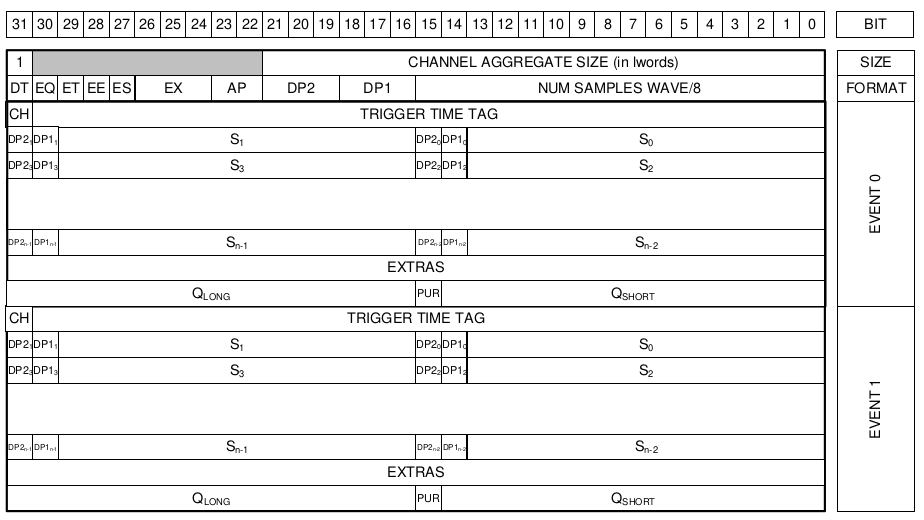
\includegraphics[scale=0.36]{Chapter-5/figs/ChannelAgg.png}
\caption{The data format for the first two events in a channel aggregate. Each memory location is 32-bits and is accessed during readout. Individual samples are not saved by our digitizer, so every 32-bit line that contains a sample, i.e. S$_{1}$, S$_{2}$, etc., is omitted. Each event therefore contains up to three memory locations. The channel aggregate itself has a header consisting of the first two memory locations - SIZE and FORMAT.}
\label{ChannelAgg}
\end{figure}

Not every bit in Figure \ref{ChannelAgg} will be discussed here. See the CAEN DPP-PSD manual for detailed information \textcolor{blue}{[Ref]}. However, the data most frequently accessed are as follows (from top to bottom in Figure \ref{ChannelAgg}). In the SIZE memory location, the CHANNEL AGGREGATE SIZE is the number of memory locations that are contained in the given channel aggregate, including itself and FORMAT. This can be useful for debugging and determining how many events are contained in the aggregate. In the FORMAT memory location, EX contains 3 bits that the user inputs (through functions in the frontend DAQ) to specify what the EXTRAS memory location outputs. See Section \ref{LED_CFD} for the specific options. If all 3 of these bits are 0, the EXTRAS memory location is omitted. In the event memory locations, CH specifies which channel the event came from in the couple (0 for even or 1 for odd). PUR is a flag that detects events whose energy was not evaluated correctly (e.g. from pile-up or event saturation). 

%Note that $Q_{\textnormal{Long}}$ and $Q_{\textnormal{Short}}$ are 16- and 15-bit signed integers, respectively, while the trigger time tag is a 31-bit unsigned integer. The reason $Q_{\textnormal{Long}}$ and $Q_{\textnormal{Short}}$ are signed integers is to clearly separate real events from noise. In the case of a pile-up event, for example,  

% (Don't use this:) Q_long and Q_short are signed integers and everything else is an unsigned integer, but the details are probably not important to include... Except that it explains the 65535 spike issue.

\subsubsection{Board Aggregate Event Format} \label{board_agg}

The board aggregates are formatted for readout as in Figure \ref{BoardAgg}. Each board aggregate contains up to 8 channel aggregates and has 4 memory locations making up the header. Each channel aggregate that has data contributes all of its memory locations to the board aggregate in the order shown in Figure \ref{BoardAgg}. Channel aggregates with no data do not contribute to the board aggregate.

\begin{figure}[b!]
\centering
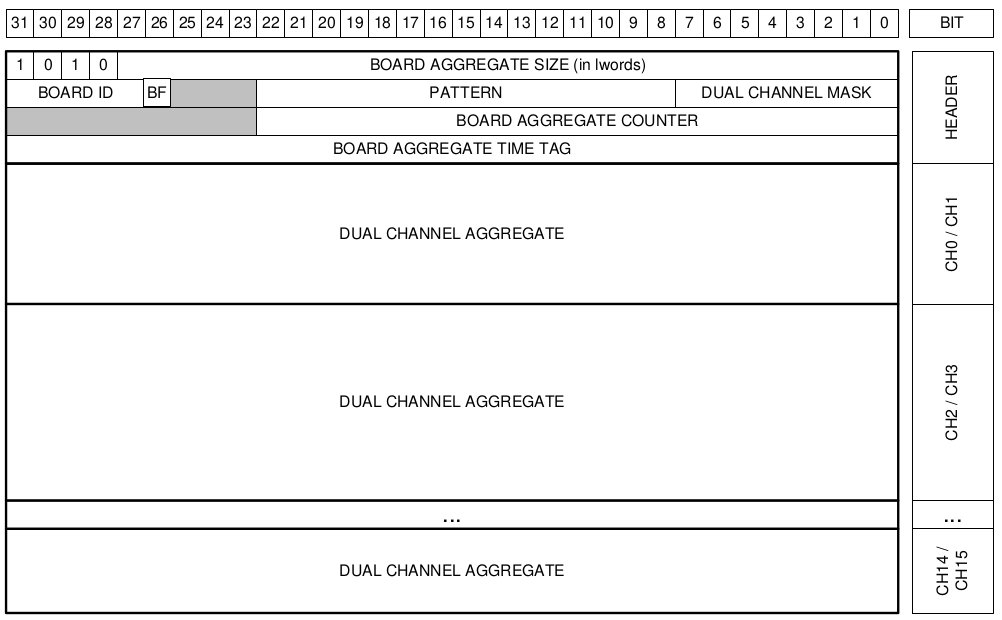
\includegraphics[scale=0.33]{Chapter-5/figs/BoardAgg.png}
\caption{The data format for a board aggregate, consisting of up to 8 channel aggregates and 4 memory locations making up the header. Each memory location is 32-bits and is accessed during readout.}
\label{BoardAgg}
\end{figure}

Again, only the most important values in the board aggregate will be discussed here. The BOARD AGGREGATE SIZE is analogous to the CHANNEL AGGREGATE SIZE in that it is the total number of memory locations contained in the board aggregate, including all of the memory locations in the channel aggregates that comprise it. The DUAL CHANNEL MASK corresponds to the channel couples participating to the board aggregate. THE BOARD AGGREGATE COUNTER gives the current board aggregate count. The BOARD AGGREGATE TIME TAG gives the time that the board aggregate was created. This is not a physical quantity, but can be useful for debugging.

%\subsubsection{Data Block} \label{data_block}

%%%%%%%%%%%%%%%%%%%%%%%%%%%%%%%%%%%%%%%%%%%%%%%%%%%%%%%%%%%%%%%%%%%%%%%%%%%%%%%

\pagebreak
\section{Frontend DAQ Software} \label{frontend}

\subsection{V1730 Registers} \label{registers}

The CAEN V1730 digitizer firmware uses Digital Pulse Processing (DPP) algorithms, which are implemented in the Field-Programmable Gate Array (FPGA) of the digitizer board. The DPP algorithms and settings can therefore be programmed by the user. This is performed by accessing and writing values to 32-bit wide \textit{registers}, which have distinct hexadecimal addresses. For example, setting the width of the long gate for channel 0 amounts to writing the long gate value (as a 16-bit integer) into the Long Gate Width register specific to channel 0, which has the address 0x1058. All of the registers that the user can access are documented in the official V1730 DPP-PSD Registers manual \textcolor{blue}{[Ref]}. %\ref{V1730 DPP Registers} 
We will highlight some of the most important ones in the next section.

An important aspect of our custom DAQ software is to provide a simple way of changing user-defined settings without the user having to manually change register values. In the DAQ software, the different settings are implemented via C++ functions that write the given parameter values into the appropriate register when executed. The function definitions are stored in the C file v1730DPP.c, while the functions are executed in the frontend C++ file fev1730-DPP.cxx. The most common settings, however, can be applied via the settings file, settings-DPP.dat.

\begin{figure}[b!]
\centering
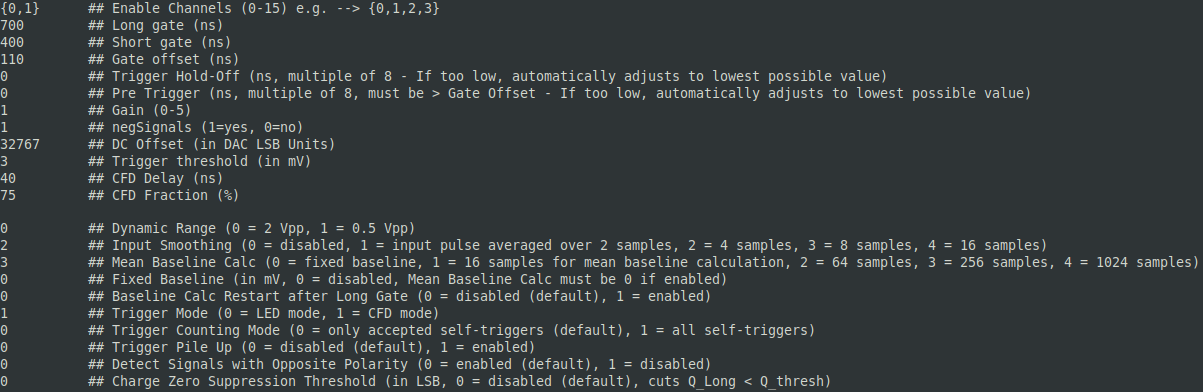
\includegraphics[scale=0.33]{Chapter-5/figs/settings_file.png}
\caption{The settings file, settings-DPP.dat, where the most common user-defined DPP parameters are adjusted. Other common V1730 register settings can be adjusted here as well.}
\label{settings_file}
\end{figure}

\subsection{User Settings} \label{settings}

\subsubsection{Settings Determined from Oscilloscope Signals} \label{oscilloscope}

\subsubsection{LED vs. CFD Mode} \label{LED_CFD}

\subsubsection{Gain} \label{gain}

\subsubsection{Mean Baseline Calculation} \label{mean_baseline_calc}

\subsubsection{Input Smoothing} \label{smoothing}

\subsubsection{Coincidences} \label{coincidences}

%Coincidences of events from different channels are obtained by subtracting their time tag values. Our DAQ has a coincidence feature that automatically deterimines coincidences between specified channels and can display coincidence spectra on the EngeSpec GUI (see

\subsubsection{Other Settings} \label{other_settings}

%\subsection{MIDAS Data Collection} \label{MIDAS} % Don't include this
\subsection{Making Changes and Starting Runs}



%%%%%%%%%%%%%%%%%%%%%%%%%%%%%%%%%%%%%%%%%%%%%%%%%%%%%%%%%%%%%%%%%%%%%%%%%%%%%%%

\pagebreak
\section{EngeSpec GUI}

\subsection{Overview of EngeSpec Operation}

\subsubsection{Sort Routine: EngeSort}

\subsubsection{Online MIDAS Runs}

\subsubsection{Offline MIDAS Runs}

\subsection{GUI Features}

\subsubsection{Histogram Display}

\subsubsection{Curve Fitting}

\subsubsection{Coincidences}

\subsubsection{Gating}

%%%%%%%%%%%%%%%%%%%%%%%%%%%%%%%%%%%%%%%%%%%%%%%%%%%%%%%%%%%%%%%%%%%%%%%%%%%%%%%

\pagebreak
\section{Examples of DAQ/EngeSpec Operation}

\subsection{Resolution Tests with a NaI Detector} \label{resolution}

\subsubsection{Energy Resolution}

\subsubsection{Timing Resolution (Coincidence Mode)}

\subsection{Coincidences with NaI Detectors}

\subsubsection{LED Mode}

\paragraph{Timing Spectrum}

\paragraph{2D Energy Spectrum}

\paragraph{2D Energy vs. Coincidence Time Spectrum}

\paragraph{Gating on Timing Spectrum}

\subsubsection{CFD Mode}

\paragraph{Timing Spectrum}

\paragraph{2D Energy Spectrum}

\paragraph{2D Energy vs. Coincidence Time Spectrum}

\subsection{Dead Time Tests with Fixed Energy Pulser}

\section{Conclusions}

